\documentclass[tikz]{standalone}
%%%\usepackage[x11names, rgb]{xcolor}
\usetikzlibrary{decorations,arrows,shapes}
\usepackage{xfrac}
\begin{document}
%%%
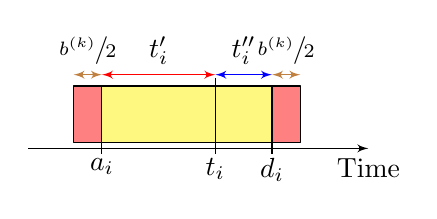
\begin{tikzpicture}[>=latex',join=bevel,domain=0.4:4.6,scale=0.72]
    \draw[->] (-1.3,0) -- (4.7,0) node[below] {Time};

    \foreach \x in {0,2,3}
     		\draw (\x,0.1) -- (\x,-0.1);

\draw (0, 0) node[below] {$a_i$};
\draw (2, 0) node[below] {$t_i$};
\draw (3, 0) node[below] {$d_i$};

\draw [<->,red]   (0,1.3) -- (2,1.3) node [black,sloped,midway,above] {$t_i^{\prime}$};

\draw [<->,blue] (2,1.3) -- (3,1.3) node [black,sloped,midway,above] {$t_i^{\prime\prime}$};

\path[draw=black,fill=yellow!50]   ( 0, 0.1) --++ (2,0) --++ (0,1) -++ (-2,0) --cycle;
\path[draw=black,fill=yellow!50]   ( 2, 0.1) --++ (1,0) --++ (0,1) -++ (-1,0) --cycle;
\path[draw=black]   ( 2, -0.05) --  (2,1.25);

\path[draw=black,fill=red!50]   ( 3, 0.1) --++ (0.5,0) --++ (0,1) -++ (-0.5,0) --cycle;
\path[draw=black,fill=red!50]   ( 0, 0.1) --++ (-0.5,0) --++ (0,1) -++ (+0.5,0) --cycle;


\draw [<->,brown]   (-0.5,1.3) -- (0,1.3) node [black,sloped,midway,above] {$\sfrac{b^{(k)}}{2}$};

\draw [<->,brown]   (3,1.3) -- (3.5,1.3) node [black,sloped,midway,above] {$\sfrac{b^{(k)}}{2}$};

\end{tikzpicture}
\end{document}